\documentclass{beamer}
\usepackage[utf8]{inputenc}
\usepackage[T1]{fontenc}
\usepackage{lmodern}
\usepackage{tabularx}
\usepackage{graphicx}
\usepackage{hyperref}
\usepackage[ngerman]{babel}

\usetheme{Antibes}

\begin{document}
\title{Zwischenpr\"asentation Geek-Shop}
\author{SWT14W30}
\date{27. November 2014}

\begin{frame}
\titlepage
\end{frame}

\begin{frame}
\frametitle{Gruppenmitglieder}
\begin{tabular}{rp{10cm}}
Chefprogrammierer: & Sebastian Döring \\
Assistent: & Elizaveta Ragozina \\
Sekretär: & Marcus Kammerdiener \\
Tester: & Dominik Lauck \\
Administrator: & Felix Döring \\[.5cm]
\textbf{Vortragender:} & \textbf{Name}\\
\end{tabular}

\end{frame}


\begin{frame}
\frametitle{Inhaltsverzeichnis}\
\tableofcontents
\end{frame}

\section{Erkl\"arung}
\begin{frame}
\begin{itemize}
\item bla
\item bla
\item bla
\end{itemize}
\end{frame}

\subsection{Bild zur Erkl\"arung}
\begin{frame}
\center{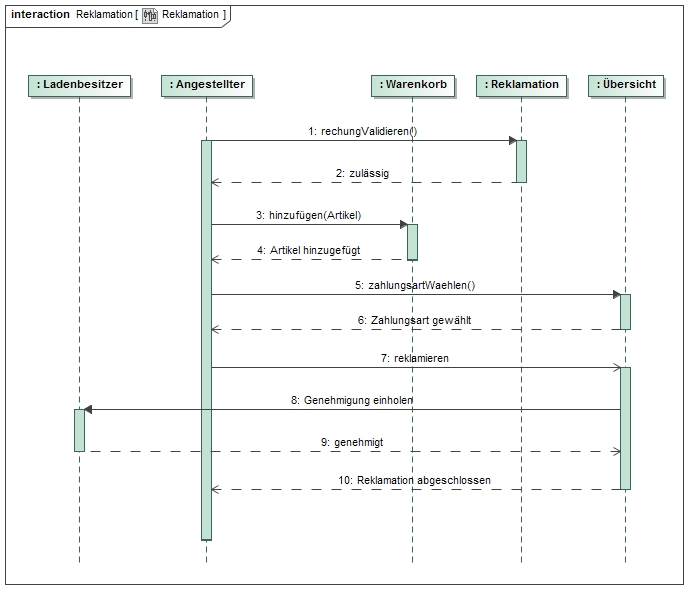
\includegraphics[scale=.3]{../Pflichtenheft/images/reklamation}}
\end{frame}



\end{document}
